\documentclass{article}

\usepackage{url} 

\usepackage{pdfpages}
\usepackage{lastpage}
\usepackage{fancyhdr}
\usepackage{ngerman}
\usepackage{listings}

\usepackage{floatrow}
\usepackage[tableposition=top]{caption}
\floatsetup[table]{capposition=top}

\usepackage{amsmath, amssymb}

\usepackage[utf8]{inputenc}


\usepackage[numbib]{tocbibind}



\newcommand\twodigits[1]{%
   \ifnum#1<10 0#1\else #1\fi
}



\lhead{Gitter, Prisma}
\rhead{9. Oktober 2020\\T. Maier, J. Winkler}
%\cfoot{\twodigits{\thepage}~/ \pageref{LastPage}}
\cfoot{{\thepage}~/ \pageref{LastPage}}

\begin{document}

\parindent0cm

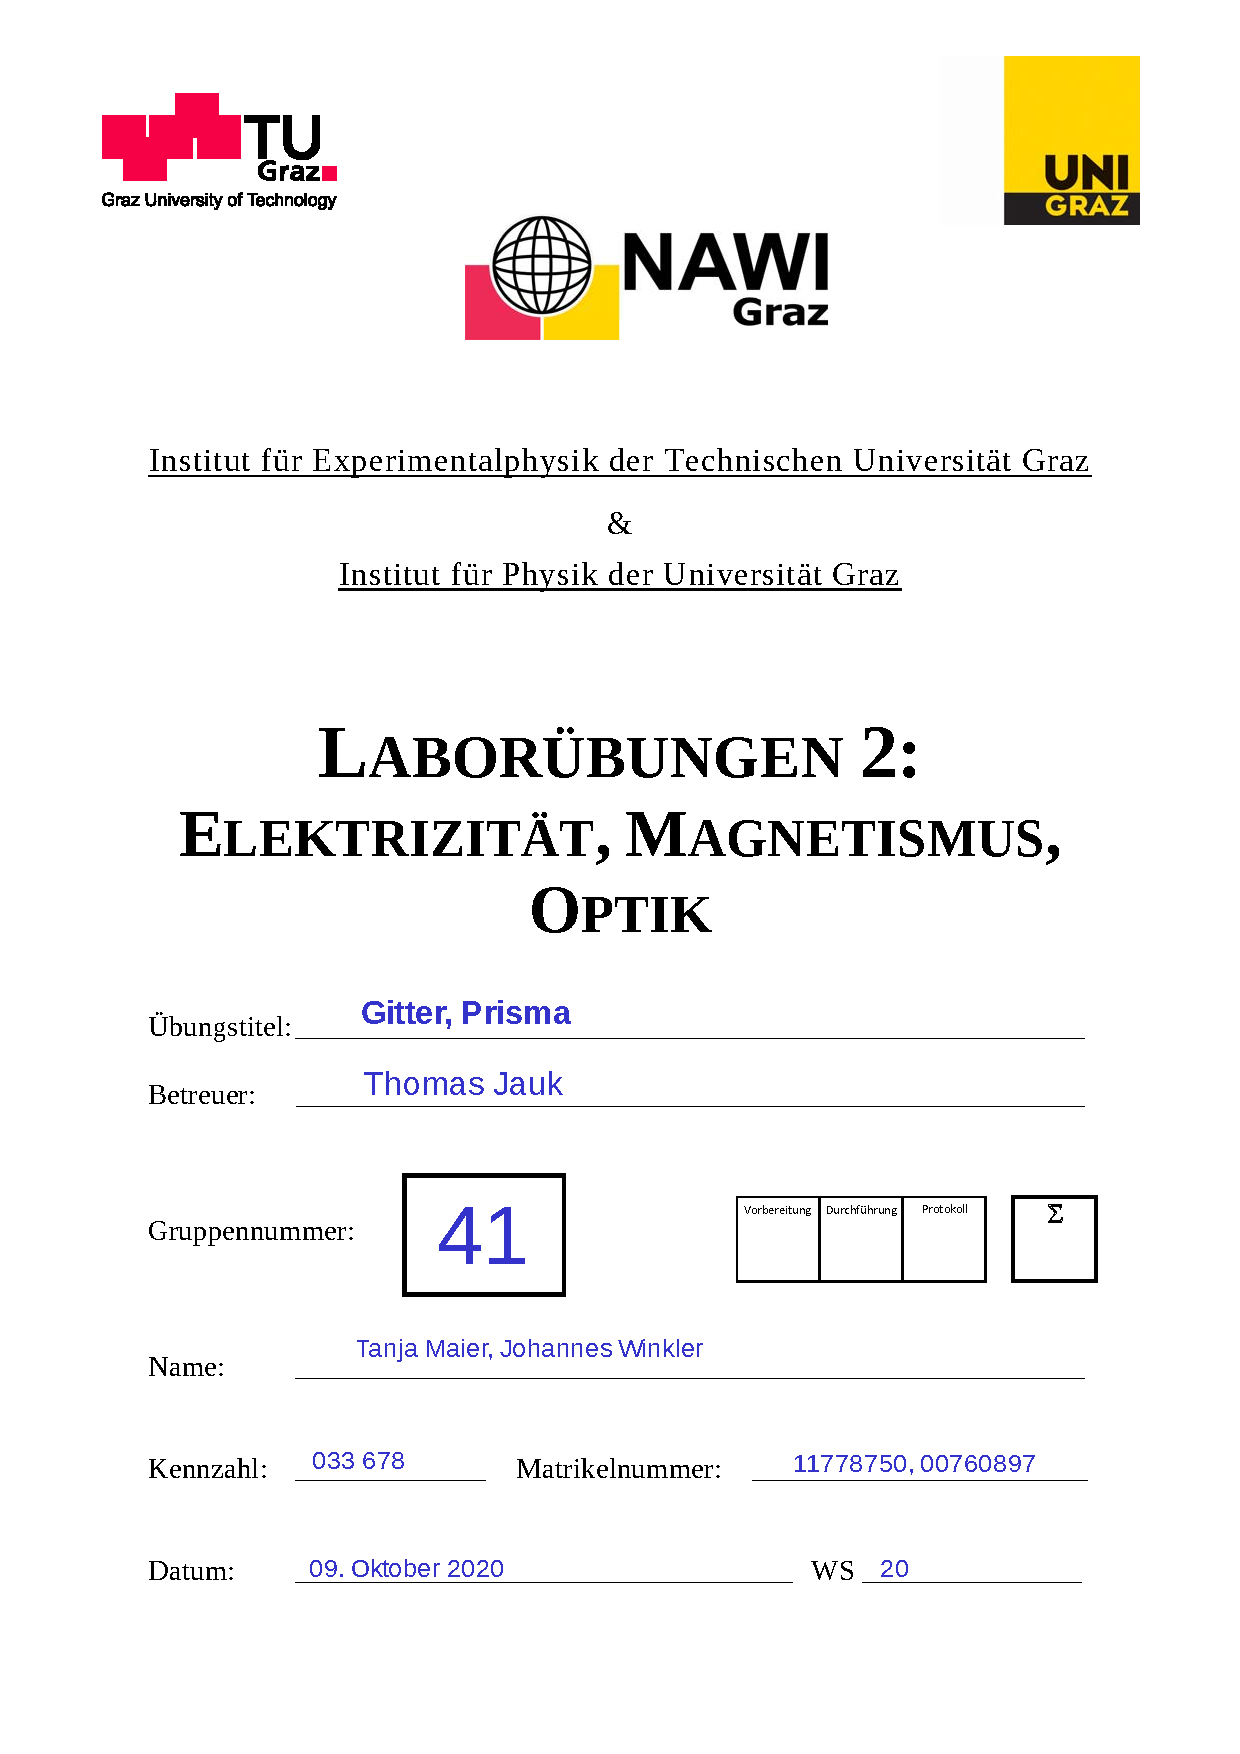
\includepdf{Deckblatt.pdf}


\pagestyle{fancy}

\section{Aufgabenstellung}

Gitter:
\begin{enumerate}
\item Justieren des Spektrometers
\item Bestimmng der Gitterkonstanten mittels Na-Dampflampe. Die Wellenlängen der gelben NA-Doppellinien sind 588.995~nm und 589.592~nm. Messung erfolgt in 2. Ordnungund wird 5 mal nach links und rechts ausgeführt. Auswertung durch Mittelwert und Standardabweichung. Bestimmung der Gitterkonstante durch Formel \eqref{eq:gitterkonst}
\item Bestimmung der Wellenlängen der gut sichtbaren Linien der Hg-Lampe. 5 Farben sollen dabei ausgewählt werden. Messungen erfolgen in 2. Ordnung einmal links und einmal rechts. Formel \eqref{eq:gitterkonst} wird zur Bestimmung der Wellenlängen genutzt.
\item Berechnung des Auflösevermögens des Gitters mit Formel \eqref{eq:aufl_gitter}
\end{enumerate}


Prisma: 
\begin{enumerate}
\item Justieren des Spektrometers
\item Bestimmung des brechenden Winkels des Prismas durch Messung des Reflexionswinkels. Messung 5 mal links und 5 mal rechts. Statistische Auswertung mit Mittelwert und Standardabweichung. Formel 22
\item Bestimmung des Brechungsindex/Dispersionskurve $n(\lambda)$ des Prismas für 5 sichtbare Linien einer Hg-Lampe nach der Methode der minimalen Ablenkung. Messung links und rechts ausführen ($\delta = \omega/2$). Mit Hilfe der formel 17 kann der Brechungsindex für die jeweilige Spektrallinie berechnet werden. Dispersionskurve plotten! Fehlerbalken!
\end{enumerate}


\section{Grundlagen und Versuchsaufbau}

\subsection{Gitter}

Ein ebenes Strichgitter besteht aus lichtdurchlässigen Öffnungen und lichtundurchlässigen Balken, welche in genau gleichen Abständen abwechselnd aufeinander folgen. Fällt Licht auf ein solches Gitter, so wird es gebeugt und gemäß dem Huygens'schen Prinzip gehen von jedem Punkt einer Öffnung Kugelwellen aus, die sich je nach der Richtung und der Wellenlänge durch Interferenz verstärken oder schwächen.

Ein Maximum der Lichtintensität in der Richtung $\phi$ wird dann beobachtet, wenn ein Bündel parallelen Lichtes senkrecht auf das Gitter trifft und der Gangunterschied $\Delta$ zwischen zwei von benachbarten Gitteröffnungen ausgehenden Elementarwelle dabei ein ganzzahliges Vielfaches der Wellenlänge $\lambda$ ist.

Somit ergibt sich die Bedingung für das Helligkeitsmaximum der Wellenlänge $\lambda$

\begin{align}
\Delta &= g\cdot \sin(\phi) \\
\label{eq:gitterkonst}
z\cdot \lambda &= g\cdot \sin(\phi)
\end{align}

wobei $z$ die Ordnungszahl des Beugungsmaximums, $\lambda$ die Wellenlänge des Lichts und $g$ der Abstand zwischen zwei Gitteröffnungen (Gitterkonstante) ist.

Für unterschiedliche Wellenlängen (d.h. unterschiedliche Farben) des einfallenden Lichts ergibt sich also eine Abfolge an Beugungsmaxima, die man als Spektrum bezeichnet. Die Ordnungszahlen $z = 1,2,3, \dots$ entsprechen dabei den Spektren 1., 2., 3. Ordnung. Je höher die Ordnungszahl $z$ ist, desto größer ist der Einfallswinkel $\phi$. Spektren verschiedener Ordnung können sich auch überdecken, da zum gleichen Winkel $\phi$ Beugungsmaxima verschiedener Ordnung für verschiedene Wellenlängen gehören.



Die Fähigkeit, zwei verschiedene Wellenlängen im Abstand $\Delta\lambda$ noch getrennt zu beobachten wird Auflösungsvermögen genannt und kann mit einem Gitterspektrographen berechnet werden. Dabei gilt die Beziehung
\begin{align}
\label{eq:aufl_gitter}
\frac{\lambda}{\Delta \lambda} = z\cdot N = \frac{z\cdot D}{g} =  \frac{b}{g}
\end{align}
wobei $z$ wieder die Ordnungszahl und $N$ die Anzahl aller vom Licht getroffenen Gitterstriche ist. Das Auflösungsvermögen nimmt proportional zur Ordnung des Spektrums und zur Anzahl der beleuchteten Gitterstriche zu.



\begin{figure}[H]
\centering
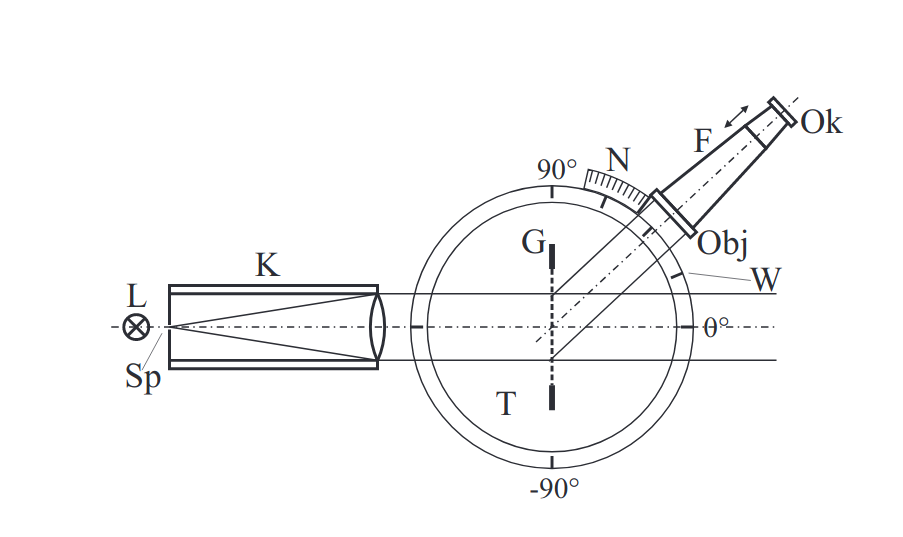
\includegraphics[scale=1.5]{gitter.png}
\caption{Aufbau zur Messung mit dem Gitter.}
\label{fig:gitter}
\end{figure}


\subsection{Prisma}

Der Brechungsindex $n$ eines Mediums ist das Verhältnis der Lichtgeschwindigkeit $c$ im Vakuum zur Lichtgeschwindigkeit $u$ im Medium
\begin{align*}
n = \frac{c}{u}
\end{align*}

Beim Übergang von einem Medium in das andere wird der Lichtstrahl gebrochen bzw. reflektiert, wenn die Medien unterschiedliche Brechungsindizes (Ausbreitungsgeschwindigkeit im jeweiligen Medium) besitzen. Dabei gilt das Brechungsgesetz von Snellius
\begin{align*}
n_1\cdot\sin(\alpha) = n_2\cdot\sin(\beta)
\end{align*}
Der Brechungsindex des Vakuums wird dabei mit $n_0 = 1$ definiert. Die Abhängigkeit $n(\lambda)$ des Brechungsindex eines Mediums von der Wellenlänge wird als Dispersionskurve bezeichnet, die Ableitung als Dispersion $D$ bei der Wellenlänge $\lambda$.
\begin{align*}
D = \frac{dn}{d\lambda}
\end{align*}
Das Auflösungsvermögen eines Prismas ist durch
\begin{align*}
\frac{\lambda}{\Delta\lambda} = t\cdot \frac{dn}{d\lambda}
\end{align*}
gegeben, wobei $t$ die Basislänge des wirksamen Strahlenbündels im Prisma darstellt ist.

Der Brechungswinkel hängt daher nicht nur vom Einfallswinkel, sondern auch von der Wellenlänge des Lichts ab - mehrfarbiges Licht (also unterschiedliche Wellenlängen) wird bei der Brechung also immer in seine Bestandteile (spektral) zerlegt. Mithilfe eines Prismas kann man sowohl die Dispersion bestimmen als auch die spektralen Eigenschaften des Lichts untersuchen. Im Sonderfall des symmetrischen Strahlenganges gilt außerdem
\begin{align*}
\alpha_1 = \alpha_2 \qquad \beta_1 = \beta_2
\end{align*}
und damit
\begin{align}
\label{eq:brechung}
n = \frac{\sin\left(\frac{\gamma + \delta}{2}\right)}{\sin\left(\frac{\gamma}{2}\right)}
\end{align}


\begin{figure}[H]
\centering
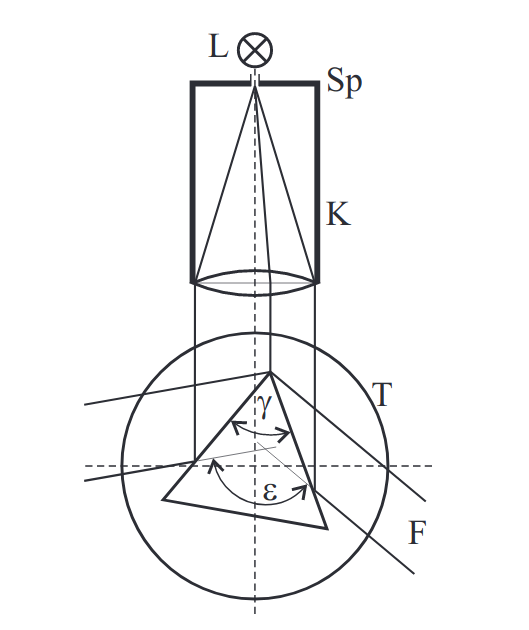
\includegraphics[scale=1.5]{prisma1.png}
\caption{Vermessung des Prismas.}
\label{fig:prisma}
\end{figure}

\newpage

\section{Geräteliste}

\begin{table}[H]
\caption{Liste der verwendeten Geräte}

~

\begin{tabular}{l|llll}
Bezeichnung & Hersteller & Typ & Inv. Nr. & Unsicherheit \\
\hline
Na-Lampe & Philips & 58230AH \\
Hg-Lampe & Philips & 40656085W \\
Spektrometer & & & V/341 \\
Gitter & & \\
Prisma & & \\
Winkelmesser & & & & $\pm~0.1~^\circ$ \\
Maßband & & & & $\pm~1~$mm
\end{tabular}

\end{table}




\section{Durchführung und Messwerte}


\subsection{Gitter mit Na-Lampe}

Zuerst wurde das Gitter in der Na-Lampe bestrahlt und währenddessen der Winkel der zwei Beugungsmaxima jeweils fünf Mal abgelesen. Nach jeder Messung wurde das Gitter kurz verschoben und die beschriebene Versuchsdurchführung wiederholt. Es wurden die inneren der beiden Linien verwendet. Die Ergebnisse sind in Tabelle \ref{tab:na_dampflampe} dargestellt.

\begin{table}[H]
\caption{Messwerte des Gitters mit Na-Dampflampe}
\label{tab:na_dampflampe}
\centering
\begin{tabular}{c|rr}
Nr. & L / ${}^\circ$ & R / ${}^\circ$ \\
\hline
1 & 172.6 & 87.7\\
2 & 172.8 & 87.7\\
3 & 172.7 & 87.7\\
4 & 172.8 & 87.7\\
5 & 172.7 & 87.7
\end{tabular}
\end{table}

\subsection{Gitter mit Hg-Lampe}

Das Gitter wurde mit der Hg-Hochdrucklampe bestrahlt. Währenddessen wurde aus dem Beugungsmaximum der Winkel von fünf verschiedenen Farben bestimmt. Die Messung wurde wieder links und rechts durchgeführt. Die Ergebnisse sind in Tabelle \ref{tab:hg_lampe} dargestellt.

\begin{table}[H]
\caption{Messwerte des Gitters mit Hg-Lampe}
\label{tab:hg_lampe}
\centering
\begin{tabular}{c|rr}
Farbe & L / ${}^\circ$ & R / ${}^\circ$ \\
\hline
Violett & 159.2 & 104.1\\
Blau & 161.7 & 101.8\\
Türkis & 166.0 & 97.6\\
Grün & 170.8 & 93.4\\
Gelb & 173.5 & 90.9
\end{tabular}
\end{table}



\subsection{Prisma}

Das Prisma wurde von der Hg-Hochdrucklampe bestrahlt und der Reflexionswinkel jeweils fünf Mal links und fünf Mal rechts gemessen. Die Ergebnisse sind in Tabelle \ref{tab:hg_lampe_prisma} dargestellt.


\begin{table}[H]
\caption{Messwerte des Prismas mit Hg-Lampe}
\label{tab:hg_lampe_prisma}
\centering
\begin{tabular}{c|rr}
Nr. & L / ${}^\circ$ & R / ${}^\circ$ \\
\hline
1 & 54.5 & 174.6\\
2 & 54.4 & 174.7\\
3 & 54.5 & 174.5\\
4 & 54.5 & 174.6\\
5 & 54.4 & 174.6
\end{tabular}
\end{table}

Dann wurde das Prisma durch Hin- und Herschwenken an der Stelle der minimalen Ablenkung (Umkehrung des Drehsinnes) platziert und die Ablenkung von fünf gut sichtbaren Farblinien gemessen. Dieser Vorgang wurde für genauere Ergebnisse an zwei einfallenden Strahlen (links und rechts) durchgeführt. Die Ergebnisse sind in Tabelle \ref{tab:hg_lampe_prisma_2} dargestellt.

\begin{table}[H]
\caption{Messwerte der Farblinien}
\label{tab:hg_lampe_prisma_2}
\centering
\begin{tabular}{c|rr}
Farbe & L / ${}^\circ$ & R / ${}^\circ$ \\
\hline
Violett & 202.9 & 80.0\\
Indigo & 202.5 & 80.9\\
Blaugrün & 201.9 & 82.0\\
Grün & 200.8 & 82.6\\
Gelb & 199.8 & 83.0
\end{tabular}
\end{table}


\section{Auswertung}

\subsection{Gitter}
Für die Gitterkonstante gilt nach Größtfehlermethode
\begin{align*}
g = \frac{2\cdot \lambda}{\sin(\phi)}
\end{align*}
 wobei $\phi = (42.51 \pm 0.2) ~^\circ$ ist. Für die Unsicherheit gilt
\begin{align*}
\Delta g = \frac{2\cdot\Delta \lambda}{\sin(\phi)} + \frac{2\cdot\lambda}{\sin^2(\phi)}\cdot \cos(\phi)\cdot \Delta\phi
\end{align*}
sofern $\phi$, $\Delta\phi$ ins Bogenmaß umgerechnet wird. Als Fehler der Wellenlänge der Na-Lampe nehmen wir $\Delta\lambda = 1~$nm an. Insgesamt ergibt sich daraus 
\begin{align*}
g = (1.74 \pm 0.01)~{\mu}m\\
\end{align*}




Für die Wellenlänge der Farben gilt
\begin{align*}
\lambda = \frac{g\cdot \sin(\phi)}{2}
\end{align*}
und dessen Unsicherheit ist
\begin{align*}
\Delta \lambda = \frac{\Delta g\cdot \sin(\phi)}{2} + \frac{g\cdot \cos(\phi)\cdot \Delta\phi}{2}
\end{align*}



\begin{table}[H]
\caption{Auswertung der Wellenlängen mit der Hg-Lampe}
\label{tab:hg_lampe_auswertung}
\centering
\begin{tabular}{c|rr}
Farbe & $\lambda$ / nm  & $\Delta\lambda$ / nm \\
\hline
Violett & 403 & 5\\
Blau & 435 & 5\\
Türkis & 490 & 5\\
Grün & 545 & 5\\
Gelb & 576 & 5
\end{tabular}
\end{table}


Die Auflösung des Gitters ist
\begin{align*}
\texttt{res} = \frac{b}{g} 
\end{align*}
mit der Unsicherheit
\begin{align*}
\Delta\texttt{res} = \frac{\Delta b}{g} + \frac{b}{g^2}\cdot\Delta g
\end{align*}

Die Vermessung der Blende hat $b=2.1~$cm ergeben, wobei beachtet werden musste, dass das Gitter nicht beschädigt wird. Desewgen ist die Messung ungenau mit $\Delta b = 0.3~$cm.
Insgesamt ergibt sich für die Auflösung
\begin{align*}
\texttt{res} = (1.2 \pm 0.2)\cdot 10^4\\
\end{align*}



\subsection{Prisma}

Zuerst wurde der brechende Winkel $\gamma$ aus den Messungen des Reflexionswinkels berechnet. Hierbei handelt es sich um die Hälfte der Differenz der Werte aus Tabelle \ref{tab:hg_lampe_prisma}. Es ergibt sich 
\begin{align*}
\gamma = 60.07~^\circ
\end{align*}

Wobei $\epsilon$ der Mittelwert der differenzierten Messungen aus Tabelle \ref{tab:hg_lampe_prisma} ist. Zum Fehler von $\gamma$ kann man sagen, dass jeder Wert aus Tabelle \ref{tab:hg_lampe_prisma} die Unsicherheit $\pm~0.1~^\circ$ hat. Die Differenz aus zwei Werten hat demnach die Unsicherheit $\pm~0.2~^\circ$. Gemäß angewandter Statistik muss man bei einem Mittelwert die Standardabweichung der einzelnen Größe durch die Wurzel der Anzahl der gemittelten Werte dividieren. Es ergibt sich daher eine Unsicherheit von $\pm~\frac{0.2~^\circ}{\sqrt{5}} \approx \pm~0.89$. Insgesamt erhält man daher für $\gamma$
\begin{align*}
\gamma = (60.07 \pm 0.89)~^\circ
\end{align*}







Dann wurde der Brechungsindex der einzelnen Farben mithilfe von Formel \eqref{eq:brechung} berechnet. Die Winkel $\delta$ wurden dabei in der Einheit Radianten eingesetzt. Die Fehlerrechnung erfolgt durch die Größtunsicherheitsmethode.
\begin{align*}
n &= \frac{\sin\left(\frac{\gamma + \delta}{2}\right)}{\sin\left(\frac{\gamma}{2}\right)} \\
\Delta n &= \frac{\cos\left(\frac{\gamma + \delta}{2}\right)}{\sin\left(\frac{\gamma}{2}\right)}\cdot \frac{\Delta \delta}{2} + \frac{\cos\left(\frac{\gamma + \delta}{2}\right)\cdot \sin\left(\frac{\gamma}{2}\right) - \sin\left(\frac{\gamma + \delta}{2}\right)\cdot \cos\left(\frac{\gamma}{2}\right)}{\sin\left(\frac{\gamma}{2}\right)} \cdot\frac{\Delta \gamma}{2}
\end{align*}
Die Ergebnisse sind in Tabelle \ref{tab:prisma_brechung}.


\begin{table}[H]
\caption{Berechnung des Brechungsindex}
\label{tab:prisma_brechung}
\centering
\begin{tabular}{c|rrr}
Farbe &  n & $\Delta n$ \\
\hline
Violett  & 1.743 & 0.001\\
Indigo  & 1.738 & 0.001\\
Blaugrün  & 1.730 & 0.001\\
Grün  & 1.723 & 0.001\\
Gelb  & 1.717 & 0.001
\end{tabular}
\end{table}


Mit den gegebenen Werten für $n$ und $\lambda$ kann eine Dispersionskurve gezeichnet werden.
\begin{figure}[H]
\label{fig:dispersion}
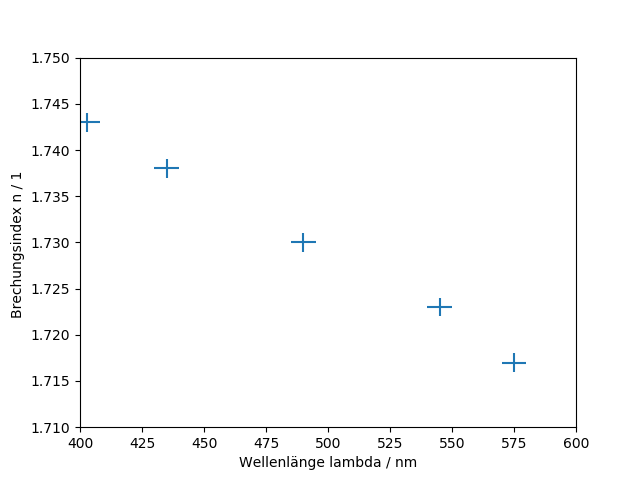
\includegraphics[scale=0.7]{kurve.png}
\caption{Dispersionskurve}
\end{figure}

\section{Zusammenfassung und Diskussion}

Für die Gitterkonstante ergibt sich
\begin{align*}
g = (1.74 \pm 0.01)~{\mu}m\\
\end{align*}


Für die Wellenlängen der Hg-Lampe gilt zusammenfassend
\begin{table}[H]
\caption{Auswertung der Wellenlängen mit der Hg-Lampe}
\centering
\begin{tabular}{c|rr}
Farbe & $\lambda$ / nm  & $\Delta\lambda$ / nm \\
\hline
Violett & 403 & 5\\
Blau & 435 & 5\\
Türkis & 490 & 5\\
Grün & 545 & 5\\
Gelb & 576 & 5
\end{tabular}
\end{table}

Für das Auflösungsvermögen des Gitters gilt
\begin{align*}
\texttt{res} = (1.2 \pm 0.2)\cdot 10^4\\
\end{align*}


Der Winkel des Prismas ist
\begin{align*}
\gamma = (60.07 \pm 0.89)~^\circ
\end{align*}



Für die Brechungsindizes gilt zusammenfassend
\begin{table}[H]
\caption{Zusammenfassung der Brechungsindizes}
\centering
\begin{tabular}{c|rrr}
Farbe &  n & $\Delta n$ \\
\hline
Violett  & 1.743 & 0.001\\
Indigo  & 1.738 & 0.001\\
Blaugrün  & 1.730 & 0.001\\
Grün  & 1.723 & 0.001\\
Gelb  & 1.717 & 0.001
\end{tabular}
\end{table}




Die gemessenen Wellenlängen liegen verglichen mit den Literaturwerten \cite{other} in einem akzeptablen Bereich.
Da es sich beim Prisma um ein gleichschenkliges Dreieck handelt, passt der berechnete Wert gut zum aufgrund der Geometrie erwarteten Wert von 60~${}^\circ$.
Auch der Brechungsindex des Prismas stimmt sehr gut mit den gefundenen Literaturwerten \cite{wiki} überein. Da sich der Brechungsindex in einem Bereich um $1.7$ befindet lässt sich sogar sagen, dass das Prisma vermutlich aus Flintglas bzw. Schwerflintglas hergestellt wurde.




\begin{thebibliography}{9}
\bibitem{other} \url{https://www.tabelle.info/farben.htm}, 11.10.2020 19:52 Uhr
\bibitem{wiki} \url{https://de.wikipedia.org/wiki/Optisches_Glas}, 11.10.2020 19:55 Uhr
\end{thebibliography}


%\newpage 
%\appendix
%\section{Python Skript}



\definecolor{commentgreen}{RGB}{2,112,10}
\definecolor{eminence}{RGB}{108,48,130}
\definecolor{weborange}{RGB}{255,165,0}
\definecolor{frenchplum}{RGB}{129,20,83}

\lstdefinelanguage{python}{
    morekeywords={def, for, range, abs, return},
    otherkeywords={<-,->, |>, \%\{, \}, \{, \, (, )},
    sensitive=true,
    morecomment=[l]{\#},
    morecomment=[n]{/*}{*/},
    morecomment=[s][\color{purple}]{:}{\ },
    morestring=[s][\color{orange}]"",
    commentstyle=\color{commentgreen},
    keywordstyle=\color{eminence},
    stringstyle=\color{red},
	basicstyle=\ttfamily,
	breaklines,
	showstringspaces=false,
	frame=tb
}
%\lstinputlisting[language=Python,captionpos=b, label=lst:test,caption={Laplace Auswertung}]{generate_numbers_laplace.py}

%\lstinputlisting[language=Python,captionpos=b, label=lst:test,caption={Bessel Auswertung}]{generate_numbers_bessel.py}


%\lstinputlisting[language=Python,captionpos=b, label=lst:test,caption={Zerstreuungslinse Auswertung}]{generate_numbers_zerstreuungslinse.py}




\end{document}
